\section{Further W+MET models with possible cross-section enhancements} 

%Contributed by Yang Bai

As pointed out in Ref.~\cite{Bell:2015sza}, the mono-$W$ signature can probe the iso-spin violating interactions of dark matter with quarks. The relevant operators after the electroweak symmetry breaking is 
%
\begin{equation}
\frac{1}{\Lambda^2}\overline{\chi} \gamma_\mu \chi \left( \overline{u}_L \gamma^\mu u_L + \xi \bar{d}_L \gamma^\mu d_L \right) \,.
\end{equation}
%
Here, we only keep the left-handed quarks because the right-handed quarks do not radiate a $W$-gauge boson from the weak interaction. As the LHC constraints the cutoff to higher values, it is also important to know the corresponding operators before the electroweak symmetry. At the dimension-six level, the following operator
%
\begin{equation}
\frac{c_6}{\Lambda^2}\overline{\chi} \gamma_\mu \chi \,\overline{Q}_L \gamma^\mu Q_L 
\end{equation}
%
conserves iso-spin and provides us $\xi=1$~\cite{1503.07874}. At the dimension-eight level, new operators appear to induce iso-spin violation and can be
%
\begin{equation}
\frac{c^d_8}{\Lambda^4}\overline{\chi} \gamma_\mu \chi \,(H\overline{Q}_L) \gamma^\mu (Q_L H^\dagger) 
+ \frac{c^u_8}{\Lambda^4}\overline{\chi} \gamma_\mu \chi \,(\tilde{H}\overline{Q}_L) \gamma^\mu (Q_L \tilde{H}^\dagger)  \,.
\end{equation}
% 
After inputting the vacuum expectation value of the Higgs field, we have 
\begin{equation}
\xi = \frac{c_6 \,+\, c_8^d\,v_{\rm EW}^2/2\Lambda^2}{c_6 \,+\, c_8^u \,v_{\rm EW}^2/2\Lambda^2} \,.
\end{equation}
% 
For a nonzero $c_6$ and $v_{\rm EW} \ll \Lambda$, the iso-spin violation effects are suppressed. On the other hand, the values of $c_6$, $c^d_8$ and $c^u_8$ depend on the UV-models. 

There is one possible UV-model to obtain a zero value for $c_6$ and non-zero values for $c^d_8$ and $c^u_8$. One can have the dark matter and the SM Higgs field charged under a new $U(1)^\prime$. There is a small mass mixing between SM $Z$-boson and the new $Z^\prime$ with a mixing angle of ${\cal O}(v_{\rm EW}^2/M^2_{Z^\prime})$. After integrating out $Z^\prime$, one has different effective dark matter couplings to $u_L$ and $d_L$ fields, which are proportional to their couplings to the $Z$ boson. For this model, we have $c_6=0$ and 
 %
\begin{equation}
\xi = \frac{-\frac{1}{2} + \frac{1}{3} \sin^2{\theta_W} }{ \frac{1}{2} - \frac{2}{3} \sin^2{\theta_W}} \approx  -2.7 
\end{equation}
%
and order of unity. 

\section{Tabulated cross-sections}

\subsection{Higgs+MET signal, vector mediator model}

%TODO: this should be tabulated

\begin{figure}[hbpt!]
	\begin{center}
		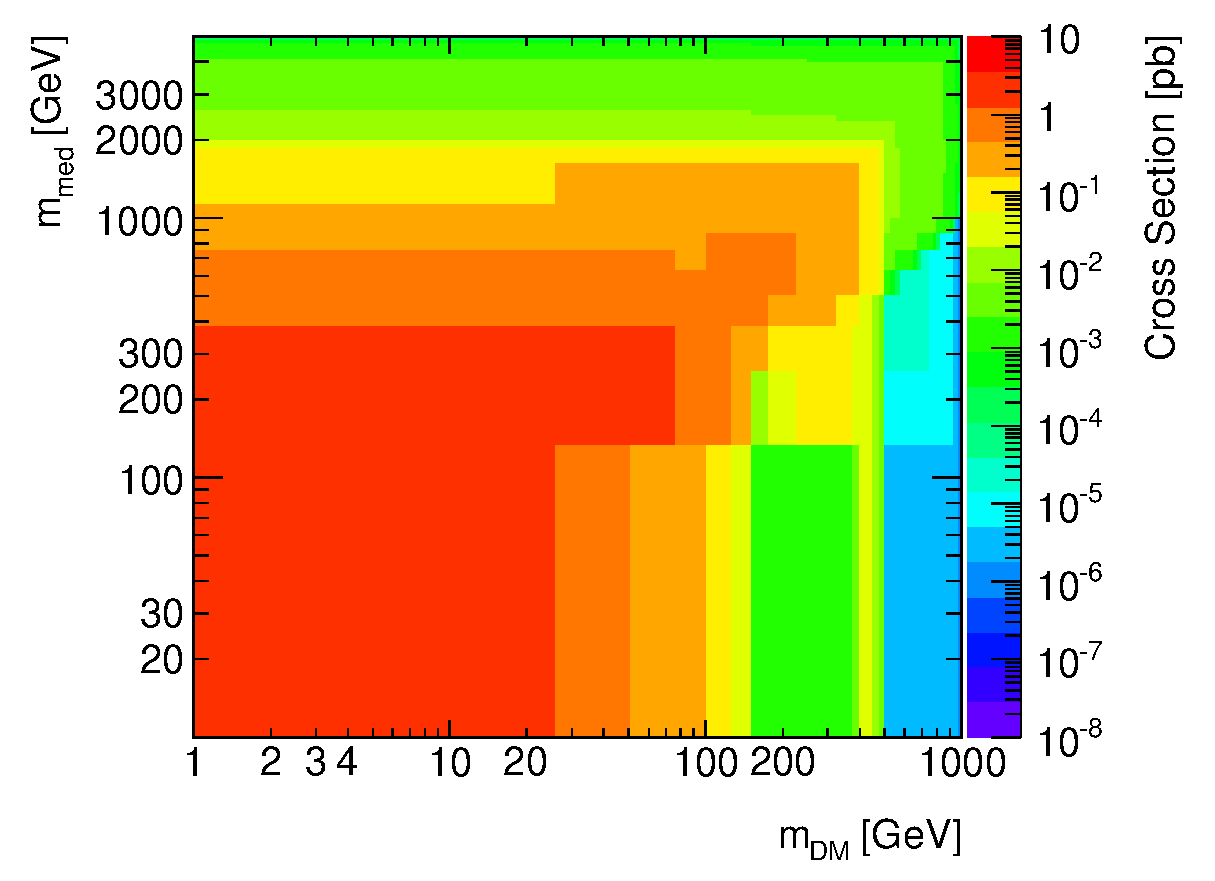
\includegraphics[width=0.9\linewidth]{figures/EW/monoH/zprime_cross_section_new}
		\caption{ Cross section of the $pp \rightarrow H\chi\bar{\chi}$ process 
			in units of pico-barn for the vector mediator model. 
			\label{fig:zprimeXS}}
	\end{center}
\end{figure}

Figure~\ref{fig:zprimeXS} shows the cross sections in this mediator model in the $m_{med}$ 
vs $m_{DM}$ plane..

\subsection{Higgs+MET signal from 2HDM model with a Z' and a new pseudoscalar}
\label{subsec:Simulation}

The leading order cross-sections from the Madgraph generator for the signal samples are listed in Tables~\ref{tab:SigSamplesZpA0}, ~ \ref{tab:SigSamplesZpDM}, ~ \ref{tab:SigSamplesZpZh}, for the various scan points recommended.  

\begin{table}
	\centering
	\small
	\begin{tabular}{|c|c|c|}
		\hline
		$M_{Z'}$ (GeV) & $M_{A^0}(GeV)$ & $\sigma$ [pb] \\ \hline \hline
		600 & 300 & 1.55E-01  \\
		600 & 400 & 2.18E-02  \\
		800 & 300 & 8.30E-02  \\
		800 & 400 & 2.72E-02  \\
		800 & 500 & 1.09E-02  \\
		800 & 600 & 2.98E-03  \\
		1000 & 300 & 3.74E-02  \\
		1000 & 400 & 1.53E-02  \\
		1000 & 500 & 8.91E-03  \\
		1000 & 600 & 4.89E-03  \\
		1000 & 700 & 2.21E-03  \\
		1000 & 800 & 7.05E-04  \\
		1200 & 300 & 1.70E-02  \\
		1200 & 400 & 7.65E-03  \\
		1200 & 500 & 5.14E-03  \\
		1200 & 600 & 3.52E-03  \\
		1200 & 700 & 2.25E-03  \\
		1200 & 800 & 1.27E-03  \\
		1400 & 300 & 8.00E-03  \\
		1400 & 400 & 3.79E-03  \\
		1400 & 500 & 2.75E-03  \\
		1400 & 600 & 2.09E-03  \\
		1400 & 700 & 1.58E-03  \\
		1400 & 800 & 1.06E-03  \\
		\hline
		\hline
	\end{tabular}
	\caption{LO cross-sections for $Z' \to A^0h$ samples, varying $M_{Z'}$ and $M_{A^0}$, keeping the DM mass fixed to 100 GeV. 
    The columns from left to right describe $M_{Z'}$, $M_{A^0}$ and the sample cross section in pb.}
   \label{tab:SigSamplesZpA0}
\end{table}

\begin{table}
	\centering
	\small
	\begin{tabular}{|c|c|c|c|}
		\hline
		$M_{Z'}$ (GeV) & $M_{A^0}(GeV)$ & $M_{DM} (GeV)$ & $\sigma$ [pb] \\ \hline \hline
		1000 & 300 & 10 & 3.76E-02  \\
		1000 & 300 & 50 & 3.75E-02  \\
		1200 & 600 & 10 & 3.64E-03  \\
		1200 & 600 & 20 & 3.07E-03  \\
		\hline
		\hline
	\end{tabular}
	\caption{LO cross-sections for $Z' \to A^0h$ samples, when varying $M_{DM}$. The columns from left to right describe $M_{Z'}$, $M_{A^0}$, $M_{DM}$, and the sample cross section in pb.}
	\label{tab:SigSamplesZpDM}
\end{table}

\begin{table}
	\centering
	\small
	\begin{tabular}{|c|c|}
		\hline
		$M_{Z'}$ (GeV) & $\sigma$ [pb] \\ \hline \hline
		600 & 1.15E-01  \\
		800 & 3.21E-02  \\
		1000 & 1.13E-02  \\
		1200 & 4.54E-03  \\
		1400 & 2.00E-03  \\
		\hline
		\hline
	\end{tabular}
	\caption{LO cross-sections for $Z' \to Zh$ exclusive samples, varying $M_{Z'}$. The columns from left to right describe $M_{Z'}$ and the sample cross section in pb.}
	\label{tab:SigSamplesZpZh}
\end{table}